Das Problem der Eisproduktionsplanung befasst sich mit folgendem Szenario:

Man besitzt eine Eis-Firma, welche über den gesamten Verlauf des Jahres Eis produzieren soll. Da man jedoch keine Über- oder Unterproduktion, und damit Verluste, in Kauf nehmen möchte, versucht man mithilfe von Vorhersagen für das folgende Jahr seine Eisproduktion hieran anzupassen. Eine mögliche Vorhersage sieht folgendermaßen aus:

\centering
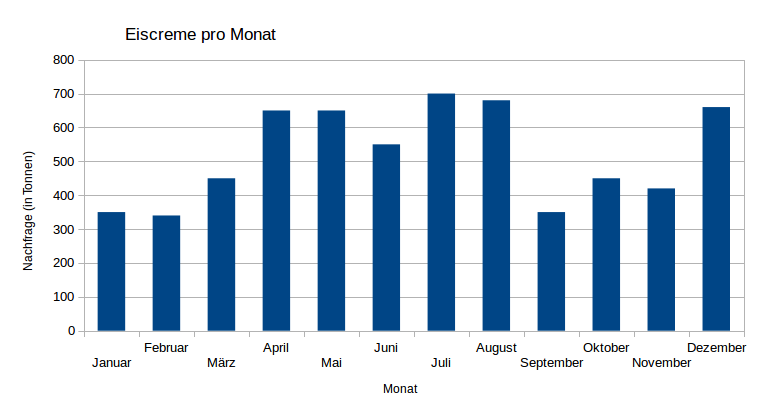
\includegraphics[width=\textwidth]{Grafiken/Eiscreme.png}

\raggedright
Bei der Erstellung der Linearen Ungleichung muss nun folgendes beachtet werden:

\begin{itemize}
\item Die Änderung der Produktionsmenge von Monat A zu Monat B kostet 50€ pro Tonne.
\item Eis lässt sich lagern, jedoch kostet dies 20€ pro Tonne pro Monat.
\item Die Produktion von einer Tonne Eis kostet 1€
\item Es darf keine Unterproduktion vorliegen, d.h. der Bedarf muss gedeckt werden.
\item Zu Anfang des Jahres gibt es kein Eis, und zu Ende des Jahres darf ebenso kein Eis mehr vorhanden sein.
\end{itemize}

Dies liefert folgende Bedingungen:
\begin{itemize}
\item Für einen Monat $m$ in $M$ muss die Produktionsmenge $p$, sowie die Menge der gelagerten Eiscreme $l$ größer als die Nachfrage $n$ sein:
\[ p_m + l_m \geq n_m \]
\item Die Menge des in einem Monat gelagerten Eises ist gleich der in vorherigen Monat übrig-gebliebenen Menge Eises:
\[ l_m = p_{m-1} + l_{m-1} - n_{m-1} \]
\item Die insgesamt produzierte Menge an Eiscreme muss gleich der gesamten Nachfrage sein:
\[ \sum p_m = \sum n_m \]
\end{itemize}

